\documentclass[a4paper,UTF8]{article}
\usepackage{ctex}
\usepackage[margin=1.25in]{geometry}
\usepackage{color}
\usepackage{graphicx}
\usepackage{amssymb}
\usepackage{amsmath}
\usepackage{amsthm}
%\usepackage[thmmarks, amsmath, thref]{ntheorem}
\theoremstyle{definition}
\newtheorem*{solution}{Solution}
\newtheorem*{prove}{Proof}
\usepackage{multirow}
\usepackage{url}
\usepackage{enumerate}
\usepackage{algorithm}
%\usepackage{ltexpprt}
\usepackage{algpseudocode}
\usepackage{amsmath}
\renewcommand{\algorithmicrequire}{\textbf{Input:}}
\renewcommand{\algorithmicensure}{\textbf{Procedure:}}
\renewcommand\refname{参考文献}

%--

%--
\begin{document}
\title{实验3. 强化学习实践}
\author{MG1733051, 庞成宾, \url{pangbin123@163.com}}
\maketitle

\section*{综述}
	强化学习是机器学习中的一个领域,强调如何基于环境而行动,以取得最大化的预期收益\cite{wiki:reinforcementLearning}。强化学习任务通常用马尔科夫决策(Markov Decision Process, 简称MDP)来描述\cite{zhou2016overview}。强化学习和监督学习的不同在于教师信号。强化学习的教师信号是动作的奖励,而监督学习的教师信号是正确的动作。

    强化学习技术是要学习一个策略。这个策略其实是一个函数,输入当前的状态$s$,输出采取动作的概率$\pi(s,a)$。监督学习希望分类器正确地对实例分类,而强化学习则希望根据当前的状态与当前的奖励和累计奖励,来获得一个较优的动作。强化学习的输入数据作为对模型的反馈,强调如何基于环境而行动,以取得最大化的预期利益。与监督室学习之间的区别在于,它并不需要出现正确的输入,输出对,也不需要精确校正次优化的行为。强化学习更加关注于在线规划,需要在探索(在未知的领域)和遵从(现有知识)之间找到平衡。

\section*{实验二   Q-learning}
	Q-learning可以用来为任何给定的有限的Markov决策过程引用提供最佳的行动选择策略。它的工作原理是学习一个动作-值函数,通常记作$Q(s,a)$,它遵循一个最优的策略,最终给出一个在状态$s$下的最优的策略\cite{wiki:qlearning}。

    该问题模型由agent,状态空间$S$和动作空间$A$组成(其中状态空间和动作空间都是离散的)。当每执行一个动作$a\in A$,agent都会有一个状态转换到另一个状态。在一个特定的状态$s$对agent进行特定的动作$a$会生成一个奖赏。则agent的目标就是最大化奖赏的和。它通过学习在每一个状态的最优的动作来达到此目标。对于每个状态来说,最优的动作是具有最高的长期奖赏的动作。这个奖赏是从当前状态开始的所有未来步骤的预期值的加权和。在具体的Q-learning算法中,只考虑了未来的一个状态的奖赏。在该算法中,定义了Q函数,该函数用来计算状态-动作对应的值(建立一个Q-Table,在该表中有状态和动作的对应关系,Q函数就是从Q-Table中取出该值)。
     \begin{align}
     Q: S \times A \rightarrow \Re.
    \end{align}

    一开始学习的时候,先初始化Q-Table,一般设置为每个元素为0,在时刻$t$,agent会通过$\varepsilon$-贪婪选择动作$a_t$,并且获得一个奖赏$r_t$和一个新的状态$s_{t+1}$,并且根据之前的状态$s_t$,新的状态$s_{t+1}$,之前的动作$a_t$和奖赏$r_t$来更新Q-Table.
     \begin{align}
     Q(s_t,a_t) \leftarrow (1-\alpha)Q(s_t,a_t)+\alpha(r_t+\gamma \max_aQ(s_{t+1},a))
    \end{align}
    具体的算法伪代码如下\cite{zhou2016overview}:

\begin{algorithm}


\hspace*{0.02in} {\bf Input:} %算法的输入, \hspace*{0.02in}用来控制位置,同时利用 \\ 进行换行
环境E;动作空间A;起始状态$x_0$;奖赏折扣$\gamma$ ;更新步长$\alpha$ .
\begin{algorithmic}[1]


\State $Q(x,a)=0, \pi (x,a)=\frac{1}{A(x)}$
$x=x_0$
\For{t=1,2,...}% For 语句,需要和EndFor对应
  \State $r,x^{\prime}=$ 在E中执行动作$a=\pi^\epsilon(x)$产生的奖赏与转移的状态;
  \State $a^{\prime}=\pi(x^{\prime});$
    \State $Q(s_t,a_t) \leftarrow (1-\alpha)Q(s_t,a_t)+\alpha(r_t+\gamma \max_aQ(s_{t+1},a))$
    \State $\pi(x)=argmax_{a^{\prime\prime}}Q(x,a^(\prime\prime);$
    \State $x=x^\prime$
\EndFor
\State \Return 策略$\pi$
\end{algorithmic}
\end{algorithm}

\subsection*{状态空间离散化}

由于Q-learning中的状态是离散的,而gym环境中状态是连续的,所以在此需要对状态空间离散化。在对状态空间离散化的过程中,首先需要确定我们连续的状态的范围,如果一个状态的某个维度的范围是无穷大,则需要给它规定一个有限的范围。其次还需要确定将状态的每一维离散化为多少个子状态。如果要离散化的状态的某一维超过了该维的范围,则将该维度离散化为对应的边界,否则,将根据范围和子状态个数n将该维度在范围之内平分n份,判断该状态落入到哪一份,即对应的离散化状态。具体的算法如下:

\begin{algorithm}

\hspace*{0.02in} {\bf Input:}
要离散化的状态$state$;离散化的空间状态范围$bounds$,要离散化的空间numSpace.
\begin{algorithmic}[1]
\State declare a list to store the result
\For{i in range(state维度)}
    \If{state[i]超过bounds[i]的的范围}
        \State 将bounds[i]的上界(超过bounds的上界)或将bounds[i]的下界存入result列表中
    \Else
        \State rangei = bounds[i][1] - bounds[i][0]
        \State offset = (numSpace[i] - 1) * bounds[i][0]/rangei
        \State scaling = (numSpace[i]-1)/rangei
        \State tempResult = int(round(scaling*state[i] - offset))
        \State result.append(tempResult)
     \EndIf
\State \Return result
\EndFor

\end{algorithmic}
\end{algorithm}

\subsection*{CartPole-v0}

在CartPole这个实验中,根据参考\cite{github:cartpole},其状态空间有四维,其中第一维是表示小车的位置,范围是[-2.4,2.4],第二维是小车的速率,大小是[-inf,inf],由于该范围是无穷大的,所以在限制其范围时,规定其范围为[-0.5,0.5],第三维是杆的角度,范围是[-41.8,41.8],单位是度,第四维是杆的顶端的速度,其范围是[-inf,inf],我将其规定为[-50,50]度。其动作空间只有两个,向左推或向右推。在离散化空间的时候,将其空间大小离散到[1,2,20,10]的大小,也就是在此不考虑小车的位移(经过调参,该设置的效果比较好,有的时候考虑小车的位移效果更差)。

在设置学习速率的时候,一开始学习的时候学习速率设置的比较大一点,然后随着episode的增加学习速率逐渐减小,同理,探索率也是在一开始的时候比较大,随着episode的增加学习速率逐渐减小。所以我将它们设置为随着episode增加而减小的函数,即$1-math.log10((t+1)/10)$,其中t是episode。损失因子设置为0.95。

在设置reward的时候,根据小车的位置和杆的角度进行设置,保证车最好在中间的位置并且小杆的角度最好为0。具体设置如下:
\begin{algorithm}

\hspace*{0.02in} {\bf Input:}
gym环境env, 观察变量state
\begin{algorithmic}[1]
\State $x,xdot,theta,thetadot = state$
\State $r1 = (env.x\_threshold - abs(x)) / env.x\_threshold - 0.8$
\State $r2 = (env.theta\_threshold\_radians - abs(theta)) / env.theta\_threshold\_radians - 0.5$
\State \Return r1+r2

\end{algorithmic}
\end{algorithm}

在实际的算法中,分为训练和测试两部分,在训练的时候,采用$\varepsilon$贪婪,而在训练部分,直接采用Q函数得出的策略。其中训练的episode为1000,测试的episode为100.由于在离散化空间的时候将小车的位置x离散的个数只有1,所以一般该实验失败的主要原因就是跑出边界。测试的reward平均值为 4099.980000, 方差为2183.923191。

\subsection*{MountainCar-v0}

在MountainCar这个实验中,根据参考\cite{github:mountaincar},其状态空间有两维,第一维是表示小车的位置,范围在[-1.2,0.6],第二维是表示小车的速度,范围在[-0.07,0.07]。动作空间有三个,向左推,不推或向右推。在离散化空间的时候,将其空间大小离散到[20,10]的大小。

在设置学习速率的时候,一开始学习的时候学习速率设置的比较大一点,然后随着episode的增加学习速率逐渐减小,同理,探索率也是在一开始的时候比较大,随着episode的增加学习速率逐渐减小。所以我将它们设置为随着episode增加而减小的函数,即$1-math.log10((t+1)/10)$,其中t是episode。损失因子设置为0.95。

在设置reward的时候,根据小车的位置进行reward,如果爬到了山顶,则给与一个好的奖励,对于一个动作,如果它推的效果比较明显(推的距离较大),则给予一个好的reward。具体设置如下:

\begin{algorithm}

\hspace*{0.02in} {\bf Input:}
gym环境env, 当前的观察变量state, 前一个观察变量stateold,是否完成done


\begin{algorithmic}[1]

\If{done=True}
\State \Return 400
\Else
\State \Return $-1/abs(state[0]-stateold[0])$
\EndIf

\State

\end{algorithmic}
\end{algorithm}

在实际的算法中,分为训练和测试两部分,在训练的时候,采用$\varepsilon$贪婪,而在训练部分,直接采用Q函数得出的策略。其中训练的episode为5000,测试的episode为100.测试的reward平均值为-150.800000, 方差为19.156453。


\subsection*{Acrobot-v1}

由于我没在网上找到具体的Acrobot-v1的介绍,所以对观察变量的含义不是很清楚。在设置离散空间大小的时候,经过多次尝试,发现[1,1,1,1,10,10]的效果还不错。

在设置学习速率的时候,一开始学习的时候学习速率设置的比较大一点,然后随着episode的增加学习速率逐渐减小,同理,探索率也是在一开始的时候比较大,随着episode的增加学习速率逐渐减小。所以我将它们设置为随着episode增加而减小的函数,即$1-math.log10((t+1)/10)$,其中t是episode。损失因子设置为0.95。

在设置reward的时候,当done,则设置一个比较大的reward,否则,保持原来的reward不变。

在实际的算法中,分为训练和测试两部分,在训练的时候,采用$\varepsilon$贪婪,而在训练部分,直接采用Q函数得出的策略。其中训练的episode为2000,测试的episode为100.测试的reward平均值为-88.600000, 方差为17.511901。



\section*{实验三 Deep Q-network}
	由于Q-learning算法作用的状态是离散的,所以对于状态空间是连续化的,则更好的学习方式是Deep Q-learning(DQN)算法。它的算法框架和Q-learning是相同的,唯一不同的是,DQN的Q函数是一个神经网络,记作$Q(s,a;\theta)$,其中$s$表示状态,$a$表示执行的动作,$\theta$就是网络的参数。DQN的目的就是得到一个Q函数网络,对于一组状态动作对$(s,a)$,是的Q函数网络的输出$Q(s,a;\theta)$等于$(s,a)$下真是的Q值。具体的算法\cite{mnih2013playing}如下:

\begin{algorithm}

\begin{algorithmic}[1]
\State Initialize replay memory D to capacity N
\State Initialize action-value function Q with random weights
\For{episode = 1, M}
   Initialize sequence $s_1={x_1}$ and preprocessed sequenced $\phi_1=\phi(s_1)$
   \For{t = 1,T}
        \State With probability $\varepsilon$ select a random action $a_t$
        \State otherwise select $a_t = max_aQ^*(\phi(s_t),a;\theta)$
        \State Execute action $a_t$ in emulator and observe reward $r_t$ and image $x_{t+1}$
        \State Set $s_{t+1} = s_t, a_t, x_{t+1}$ and process $\phi_{t+1}=\phi(s+1)$
        \State Store transition($\phi_t, a_t, r_t, \phi_{t+1}$) in $D$
        \State Sample random minibatch of transitions($\phi_j, a_j, r_j, \phi_{j+1}$) from $D$
        \If{$\phi_{j+1}$ is terminal}
            \State $y_j = r_j$
        \Else
            \State $y_j=r_j+\gamma \max_{a^\prime}Q(\phi_{j+1},a^\prime;\theta)$
        \EndIf
        \State Prefome a gradient descent step on ($y_j-Q(\phi_j,a_j;\theta)$)
   \EndFor
\EndFor
%\State \Return result
\end{algorithmic}
\end{algorithm}

我将Q值网络设置为三层的全连接层,其中具体的结构是第一层的形状是(numInputs, 8),第二层的形状是(8,16),第三层的形状是(16, numOutputs),其中numInputs是输入变量的维度,即观察变量的维度,numOutputs是输出变量的个数,即动作的个数。Q值网络的学习率是0.0005, 选择的优化器是RMSProp。

\subsection*{CartPole-v0}

在该实验中,设置M为1000,T=200, N=20000,$\epsilon$是随着episode的增加而减小的,即$1-math.log10((t+1)/10)$,其中t是episode。mini-batch的大小为32。折扣率为0.95,reward function的设置和qlearning的相同,具体可见Algorithm 3.

\begin{figure}[htb]
    \center{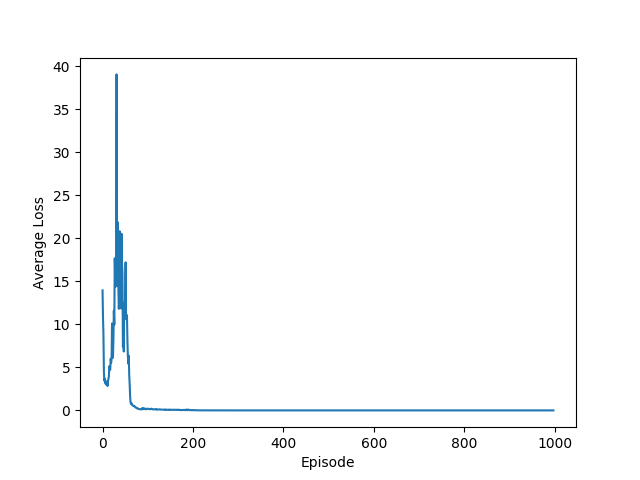
\includegraphics[width=10cm] {./pic_results/loss_dqn_cartpole.png}}
    \caption{\label{cartpole:1} CartPole训练误差岁训练轮数变化关系}
    \end{figure}

由图1可以看到,训练误差一开始处于不稳定的状态,但当训练轮数增加之后,则慢慢趋于0,证明训练效果还是挺好的。

\begin{figure}[htb]
    \center{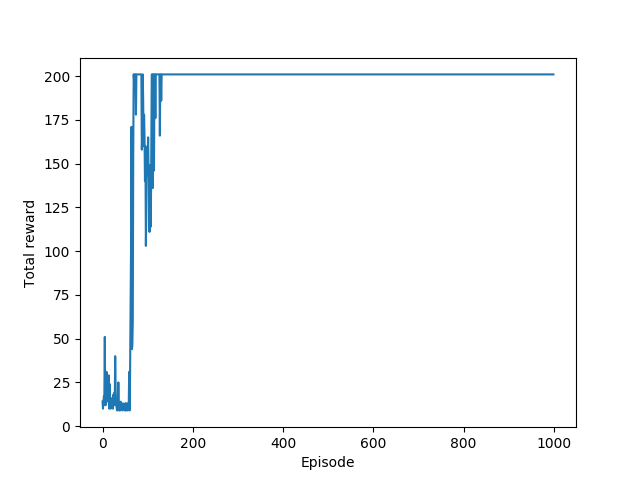
\includegraphics[width=10cm] {./pic_results/reward_dqn_cartpole.png}}
    \caption{\label{cartpole:2} CartPole每轮训练 reward之和随训练轮数的变化关系}
    \end{figure}

由于设置的T为200,所以每轮的reward之和最大为200。由图2可以看到,一开始reward之和处于不稳定状态,之后则稳定为200.

在测试的时候,设置轨迹最大长度为2000,得到reward之和的均值是20000,标准差为0.

\begin{figure}[htb]
    \center{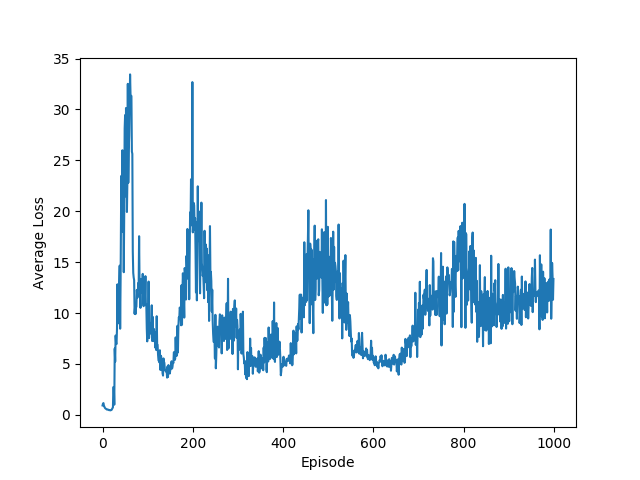
\includegraphics[width=10cm] {./pic_results/loss_dqn_mountaincar.png}}
    \caption{\label{mountainCar:1} MountainCar训练误差岁训练轮数变化关系}
    \end{figure}

\subsection*{MountainCar-v0}	
在该实验中,设置M为1000,T=500, N=20000,$\epsilon$是随着episode的增加而减小的,即$1-math.log10((t+1)/10)$,其中t是episode。minibatch的大小为32,折扣率为0.95,reward function的设置和qlearning的相同,具体可见Algorithm 4.

由图3可知,训练的误差总体上是下降的,但是不是很稳定。由图4可知,reward总体上是增加的。

\begin{figure}[htb]
    \center{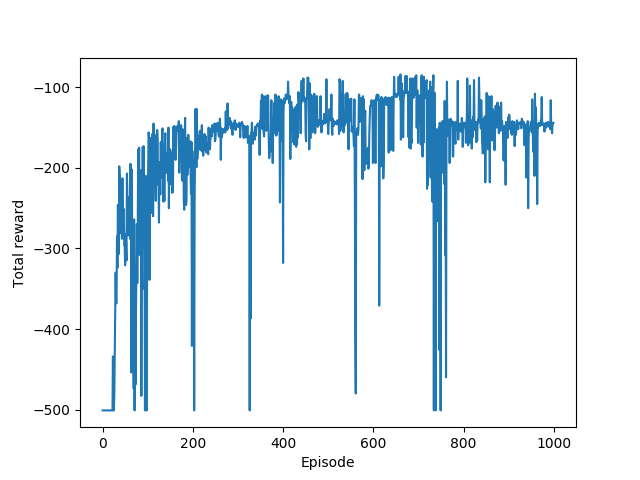
\includegraphics[width=10cm] {./pic_results/reward_dqn_mountaincar.png}}
    \caption{\label{mountainCar:2} MountainCar每轮训练 reward之和随训练轮数的变化关系}
    \end{figure}


在测试的时候,设置轨迹最大长度为2000,得到reward之和的均值是-145.220000,标准差为3.377226.

\begin{figure}[htb]
    \center{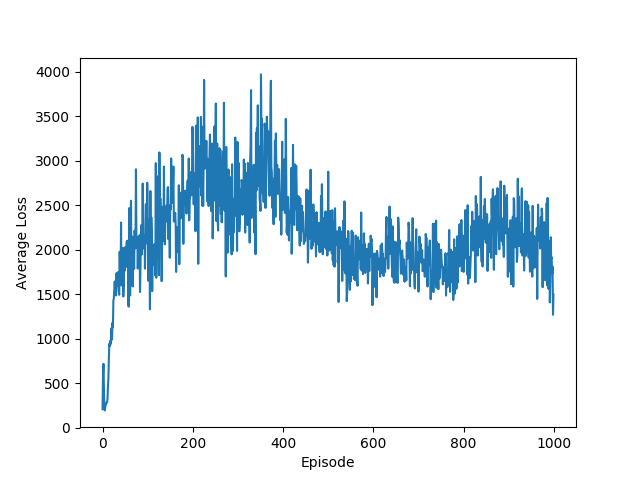
\includegraphics[width=10cm] {./pic_results/loss_dqn_acrobot.png}}
    \caption{\label{Acrobot:1} Acrobot训练误差岁训练轮数变化关系}
    \end{figure}

\subsection*{Acrobot-v1}
在该实验中,设置M为1000,T=1000, N=20000,$\epsilon$是随着episode的增加而减小的,即$1-math.log10((t+1)/10)$,其中t是episode。minibatch的大小为32,reward function的设置和qlearning的相同,折扣率为0.95.

由图5可知,训练误差随着episode的增加而呈减小趋势,不过不稳定;由图6可知,reward随着episode的增加而呈增加趋势,也不是很稳定。

\begin{figure}[htb]
    \center{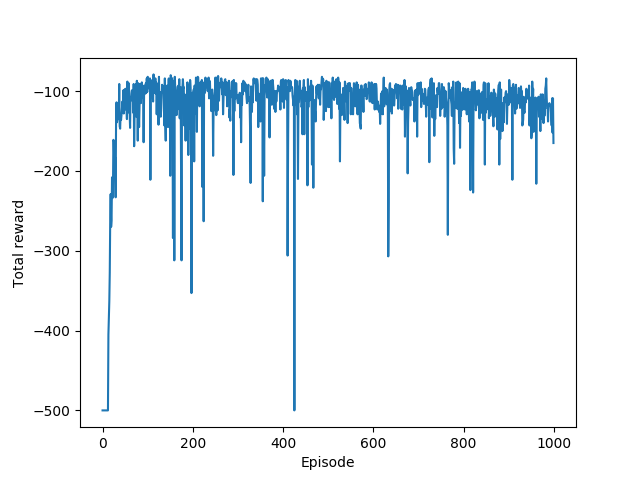
\includegraphics[width=10cm] {./pic_results/reward_dqn_acrobot.png}}
    \caption{\label{Acrobot:2} Acrobot训练误差岁训练轮数变化关系}
    \end{figure}

\section*{实验四 Improved DQN}
	在传统的DQN网络中,每探索一步都要更新一下网络的权重,而这样的更新方式可能是不稳定的\cite{mnih2015human}。该论文\cite{mnih2015human}提出的一个改进方案就是同时设置两个网络结构相同的网络,其中网络Q用来选择action和每步迭代更新,而target Q网络用来获得目标的值。每C步更新target Q为网络Q。

网络的结构和实验三的结构一样,只不过是增加了一个相同结构的target网络。

由于在DQN算法中,max操作使用同样的值来进行选择和衡量一个行动,而这实际上更可能选择过高的估计值,从而导致郭宇乐观的值估计,导致Q值较大。而在Improved DQN算法中,采用两个网络,一个网络延迟另一个网络C步更新网络参数,这样使得$y_t$更加稳定,即Q网络的目标更加稳定。

\subsection*{CartPole-v0}

\begin{figure}[htb]
    \center{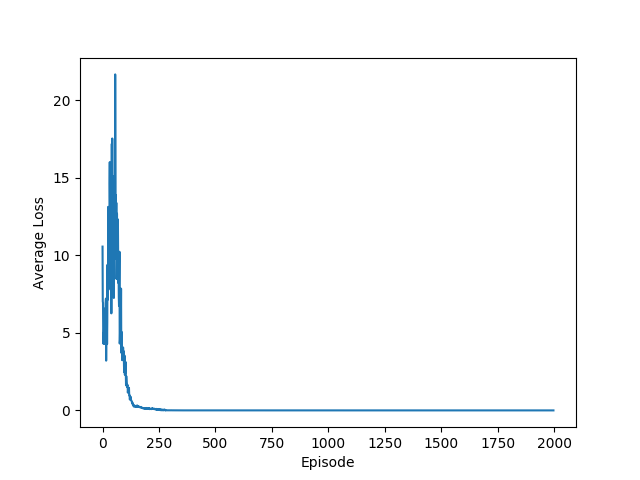
\includegraphics[width=10cm] {./pic_results/loss_Idqn_cartpole.png}}
    \caption{\label{CartPole:3} CartPole每轮训练 reward之和随训练轮数的变化关系(Improved DQN)}
    \end{figure}
在该实验中,设置M为2000,T=200, N=20000,$\epsilon$是随着episode的增加而减小的,即$1-math.log10((t+1)/10)$,其中t是episode。mini-batch的大小为32。折扣率为0.95,reward function的设置和qlearning的相同,具体可见Algorithm 3.

\begin{figure}[htb]
    \center{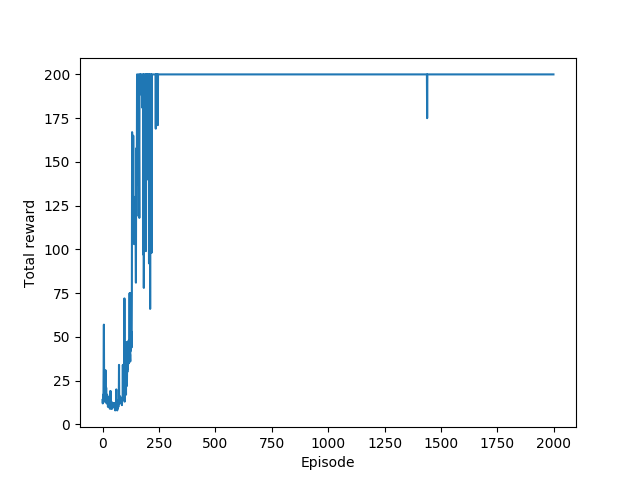
\includegraphics[width=10cm] {./pic_results/reward_Idqn_cartpole.png}}
    \caption{\label{CartPole:4} CartPole每轮训练 reward之和随训练轮数的变化关系(Improved DQN)}
    \end{figure}

由图7可以看到训练误差随着episode的增加而逐渐减小,最后趋向于0,;由图8可以看到reward之和随着episode的增加而逐渐增减,最后稳定到200.由于我的DQN的cartpole的实验结果也很理想,所以从该实验中暂未看出两个方法所产生的效果的差别。

\subsection*{MountainCar}
\bibliographystyle{plain}
\bibliography{assign3}
\end{document} 